\documentclass[a4paper]{article}
\usepackage[utf8]{inputenc}
\usepackage[natbib,sorting=none]{biblatex}
\usepackage{graphicx}
\usepackage{acronym}
\usepackage{indentfirst}
\usepackage[none]{hyphenat}
\usepackage{fancyhdr}
\usepackage{enumitem}
\usepackage{xcolor}
\usepackage{listings}
\lstset{basicstyle=\ttfamily,
  showstringspaces=false,
  commentstyle=\color{red},
  keywordstyle=\color{blue}
}

\addbibresource{references.bib}
\newcommand{\comment}[1]{\textbf{Comment: #1}}

\begin{document}
\begin{figure}[!h]
	\centering
	
\includegraphics[width=80mm]{images/poli-logo.png}
\end{figure}
\hfill
\begin{center}
    \fontsize{18px}{6mm}\selectfont \textsc{\textbf{Software Engineering II project}}
\end{center}
\begin{center}
    \fontsize{12px}{4mm}\selectfont \textsc{Academic Year: 2018/2019}
\end{center}
\hfill
\hfill
\begin{figure}[!h]
	\centering
	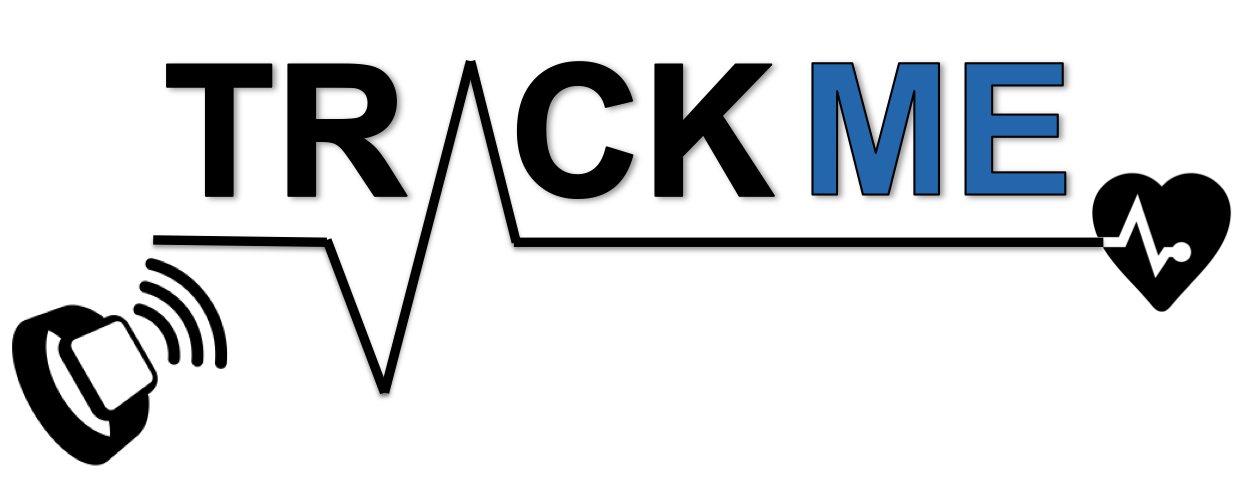
\includegraphics[width=120mm]{images/trackme-logo.png}
\end{figure}
\hfill
\hfill
\begin{center}
    \fontsize{22px}{8mm}\selectfont \textsc{\textbf{Requirement Analysis and\\ Specification Document}}
\end{center}
\begin{center}
    \fontsize{14px}{4mm}\selectfont \textsc{{Draft Version 0.1 - 11/10/2018}}
\end{center}
\hfill
\hfill
\begin{center}
\fontsize{14px}{4mm}\selectfont \textsc{\textit{Davide Rutigliano -  903616}}
\end{center}

\begin{center}
\fontsize{14px}{4mm}\selectfont \textsc{\textit{Claudio Ferrante - 903417\\}}
\end{center}

\begin{center}
\fontsize{14px}{4mm}\selectfont \textsc{\textit{Davide Matta - 903616}}
\end{center}
\pagenumbering{roman}
\tableofcontents
\newpage
\pagenumbering{arabic}
\section{Purpose and Scope}
This document is intended for presenting how all the features presented and designed in previous documents have been implemented \cite{dd}\cite{rasd}. In addition, the document be points out rationale for design choices for the adopted development frameworks.

This paper also contains a detailed description of the whole implementation both of client and server code and further testing following the \textit{I\&T plan}.

Finally, it contains all the installation and build instruction both for client and server, needed to run the code.

This document is intended for developers or anyone interested in the impleme-\newline ntation details of \textit{TrackMe}.

\section{Requirements and Functions}
This chapter is focused on highlighting requirements presented in previous documents, assuming the reader has previously read both Requirement and Design Document. In particular requirements implemented are from Data4Help and Track4Run services; AutomatedSos functionality instead has been not imple-\newline mented because not requested by the customer.

\section{Adopted Development Frameworks}

\subsection{Programming Language}
For both server and client side application the adopted language is Java: version 8 server-side, version 7 client-side; version 7 for mobile application is in order to support older OS version such as \textit{Android KitKat (4.0)}. The rationale for this choice is that Java is more suitable for large-scale application with respect to other programming languages. In addition it has a large number of libraries and frameworks and it is also supported by android, needed for the client application.

\paragraph{Pros:}

\begin{itemize}
    \item Object Oriented language
    \item Cross-Platform support
    \item Proprietary implementation of Persistence API
    \item Proprietary implementation of Authentication and Access Control
    \item Test-driven development
    \item Scalability
    \item High Performance
\end{itemize}

\paragraph{Cons:}
\begin{itemize}
    \item Code Verbosity
\end{itemize}

\subsection{Frameworks, Libraries and Other Software}

\paragraph{Server-Side Frameworks}
\begin{itemize}
    \item Spring Framework: this choice is an alternative to Java Enterprise Edition and Enterprise Java Bean based models. The main advantage of this framework is indeed that allows programmers to write less code and to focus on critical parts of the application instead of \textit{"simple and standard"} things. For instance, Spring Boot allows developers to create application with embedded web server such as Tomcat or Jetty with few lines of configuration without installing the web server itself. In addition, this framework also supports dependency injection and inversion of control. These latter features also allows developer to speed up and facilitate unit testing.
\end{itemize}

\paragraph{Client-Side Libraries}
In the Design Document we proposed Google for Map libraries, but since June 2018 Google Maps is not free anymore, we implemented our custom version  of the map\footnote{In a production system it may be better to use Google Maps API to manage maps as their libraries are widely used and tested with respect to a custom map implementation.}, using following libraries:
\begin{itemize}
    \item Osmdroid;
    \item Osmbonuspack;
    \item GraphView;
    \item StompClient\footnote{For STOMP protocol, we implemented our set of libraries in order to make it work because public libraries available online works bad or does not work at all.}.
\end{itemize}

\paragraph{Other Software}
\begin{itemize}
    \item MySQL Database as database system.
\end{itemize}

\subsection{API}
\begin{itemize}
    \item Wear OS (Android Wear) API in order to make the mobile application communicate with an external devices such as a smartwatches.
\end{itemize}

\newpage
\section{Structure of the Code}
The application has been implemented following the design document, then structure of the code is almost the same presented into component and class diagrams, with little modifications skipped in the design document in order to not overload them.

Furthermore, the overall structure of both client and server application is organized in packages in order to improve reusability and maintainability of the code.

\subsection{Server Code Packages}
\begin{itemize}
\item \textbf{config:} spring configuration classes for security and web sockets
\item \textbf{constant}
\item \textbf{model:} contains two sub-packages, first spring entities used by repositories and second DTO classes related to entities
\item \textbf{repository:} spring crud repository classes
\item \textbf{service:} spring services, the business logic of the application
\item \textbf{controller:} spring controllers, handles communications between server logic and client presentation layer
\item \textbf{token:} contains spring security token authentication filter and token utilities
\end{itemize}

\subsection{Client Code Packages}
\begin{itemize}
\item \textbf{model: models in the MVP pattern. Contains DTO classes (i.e java beans), that will contain all the data shared between server and client.}
\item \textbf{view:} views in the MVP pattern. Contains interfaces that provide the UI methods that will be implemented in every activity.
\item \textbf{presenter:} presenters in the MVP pattern. Contains logic classes that handles the communication between server and client, and other business logic.
\item \textbf{activity:} contains android activity classes that implements a view. Activities represent a single screen in the android environment.
\item \textbf{fragment:} contains android fragment classes. They are similar to activities, but they can't exist on their own. They must be instantiated inside an activity.
\item \textbf{httprequest:} contains all http logic to send and receive http messages.
\item \textbf{task:} contains android asynchronous task classes. An asynchronous task is like a new thread, that will send a callback when completed. They are used by presenters to do the business and communication logic.
\item \textbf{websocket:} contains all the websockets logic and the STOMP protocol implementation.
\item \textbf{session:} contains classes that handles the application session.
\item \textbf{util: contains utility classes, for example a factory that builds a loading screen.}
\end{itemize}

\newpage
\section{Testing}
Testing code is available within the project directory in "test" package.

\subsection{Server Side Testing}
Server-side code has been tested using the tools provided by Java with some additional libraries. In particular were used the JUnit to test the part that works in local without using external resources such as DBMS or network and Mockito, a popular mock framework which can be used in conjunction with JUnit.

\subsection{Client Side Testing}

\newpage
\section{Install Instructions}

First of all you should install git and then clone \textit{TrackMe} repository from:
\begin{lstlisting}
https://github.com/DavideRutigliano/FerranteMattaRutigliano
\end{lstlisting}

Then, to build and install the application, independently server or client, you can proceed in two different ways: build the application within your IDE or with Maven/Gradle wrapper. The latter option is widely advised, as it allows to build and run the source code without installing anything else.

\subsection{Server Build and Installation}
\begin{enumerate}
    \item Install MySQL;
    \item Create a new database schema called \textit{"trackme\_db"};
    \item Create an user with username \textit{"trackmeadmin}" identified by password \textit{"password"} with all privileges on the schema created in step 2; \item Alternatively to step 3, you can use an existing user changing
    \newline\textit{"spring.datasource.username"} and \textit{"spring.datasource.password"}\newline in \textit{"application.properties"}. 
\end{enumerate}

\subsubsection{Build with IDE}
\begin{enumerate}
    \item Open as a project: \textit{"ferrantemattarutigliano/software/server/src/pom.xml"} and wait until import is complete;
    \item Setup project sdk: file ${->}$ project structure ${->}$ project sdk (you need at least project language level 11);
    \item Add configuration ${->}$ application ${->}$ main class: ServerApplication.
\end{enumerate}

\subsubsection{Build with Maven}
With Maven wrapper you can build, install and run the application without installing any other software component, as Maven will download it for you from Maven central repository.

\paragraph{Unix:} in order to build \textit{TrackMe} server with Maven you do:

\begin{lstlisting}[language=bash]
cd FerranteMattaRutigliano/software/server
sudo chmod +x mvnw
./mvnw package
\end{lstlisting}

Then, you run the application:

\begin{lstlisting}[language=bash]
java -jar ./target/server/server-0.0.1-SNAPSHOT.jar
\end{lstlisting}

\paragraph{Windows:} in order to build \textit{TrackMe} server with Maven you do:

\begin{lstlisting}[language=bash]
cd FerranteMattaRutigliano\software\server
mvnw.cmd package
\end{lstlisting}

Then, you run the application:

\begin{lstlisting}[language=bash]
java -jar .\target\server\server-0.0.1-SNAPSHOT.jar
\end{lstlisting}

\subsection{Client Build and Installation}
In order to build client mobile application within an IDE, you should use Android Studio.

\subsubsection{Build with Android Studio}
\begin{enumerate}
    \item Download android studio;
    \item Install android studio and Android Virtual Device;
    \item Open an existing android studio project:
    \newline\textit{"ferrantemattarutigliano/software/client/build.gradle"} and wait until import is complete;
    \item Select file ${->}$ project structure. Make sure that Android NDK is installed;
    \item Run the application and create a new virtual device (you can choose the default one, Nexus 6). Select an API with version ${>=}$ 16;
\end{enumerate}

\paragraph{Known Error}
Emulator: ERROR: x86 emulation currently requires hardware acceleration!

\textbf{Solution:} tools ${->}$ SDK Manager ${->}$ SDK Tools (tab) and make sure that Intel x86 Emulator Accelerator is installed. If not, install it; if already installed, uninstall and re-install it.

\paragraph{Important Notes}
\begin{itemize}
    \item When you create the android SDK directory, don't use white space or '-' characters. This causes problem with the Android framework;
    \item If you prefer to launch the application on your own android device you can do that: enable USB debug on your android phone and connect it to your PC with an USB cable.
\end{itemize}

\subsubsection{Build with Gradle}
With Gradle wrapper you can build, install and run the application without installing any other software component, as Gradle will download it for you from Maven central repository.

\paragraph{Unix:} in order to build \textit{TrackMe} server with Gradle you do:

\begin{lstlisting}[language=bash]
cd FerranteMattaRutigliano/software/client
sudo chmod +x gradlew
./gradlew installDebug
\end{lstlisting}

\paragraph{Windows:} in order to build \textit{TrackMe} server with Gradle you do:

\begin{lstlisting}[language=bash]
cd FerranteMattaRutigliano\software\client
gradlew.bat installDebug
\end{lstlisting}

\newpage
\section{Effort Spent}
    \begin{itemize}
        \item[-] \textbf{Davide Rutigliano: }
        
        \item[-] \textbf{Davide Matta: }
        
        \item[-] \textbf{Claudio Ferrante: }
    \end{itemize}
\end{document}